\documentclass[fleqn]{beamer}
\usepackage{amsmath}
\usepackage{tikz}
\usepackage{amsmath}
\usepackage{tikz-cd}


% Presentation information
\title{What is a deterministic theory?}
\author{Hans Halvorson}
\date{January 10, 2025}

\usetheme{metropolis}

%% possibly something about "intrinsic" formulations. Think about the
%% Sider thing about theories stating relations between physical
%% objects and numbers

\begin{document}

% Title slide
\begin{frame}
    \titlepage
\end{frame}

\begin{frame}{Who cares about determinism?}

 \begin{itemize}
 \item Determinism as the enemy of human freedom and responsibility
 \item Determinism as the friend of scientific understanding,
   explanation, intelligibility, and control
 \end{itemize}


\end{frame}
  

\begin{frame}{Determinism and natural philosophy}

  ``Determinism wins our unceasing admiration in forcing to the
  surface many of the more important and intriguing issues in the
  length and breadth of the philosophy of science.'' (Earman,
  \emph{Primer of Determinism}, p 21)

  \begin{itemize}
  \item Hole argument
  \item Determinism
  \item Syntactic versus semantic view of theories
  \item Formal definitions (e.g.\ of equivalence)
  \end{itemize}  

\end{frame}

\begin{frame}{Negative perspectives}

  \begin{itemize}
  \item Unclear: Determinism is an ontological thesis (Earman 1986)
  \item Deleterious: Determinism is not a formal property of theories,
    but is a property of interpreted theories (Belot 1995)
  \item False dilemma: Determinism is a matter of semantics rather
    than syntax

  \end{itemize}

\end{frame}

\begin{frame}{Positive perspectives}

  \begin{itemize}
  \item Arrows between models are an essential part of the content of
    a theory
    \begin{itemize}
    \item Sometimes clarification calls for formal specification
    \end{itemize}
  \item Let empirical science (physics) bend and stretch our
    metaphysical frameworks
  \item Syntax as an aid in the quest for clarity
  \end{itemize}
  
\end{frame}


\begin{frame}{Definitions of determinism}

  \begin{itemize}
  \item Syntactic
    \begin{itemize}
    \item Smart
    \item Nagel
    \end{itemize}
  \item Semantic
    \begin{itemize}
    \item Montague  
    \item Lewis
    \item Earman
    \item Butterfield
      \begin{itemize}
      \item Dm1
      \item Dm2
      \end{itemize}
    \item Landsman
    \end{itemize}
  \end{itemize}

\end{frame}


\begin{frame}{What's wrong with syntactic analyses?}

  \begin{enumerate}
  \item Montague: For each time $t$, there is a distinct sentence
    $\phi _t$ that is true at $t$. But then there are uncountably many
    sentences, which is not permitted in ``standard'' languages.
  \item Earman: If we have to use an uncountably infinite signature,
    then the completness theorem fails.
  \end{enumerate}


\end{frame}

\begin{frame}{Earman against syntactic analyses}

  ``Many philosophical discussions of determinism are couched in terms
  of theories, construed as linguistic entities. But since determinism
  is a doctrine about the nature of the world, no problem is avoided
  by this linguistic detour.'' (PD, p 20)

\end{frame}

\begin{frame}{Belot against formal analyses}

  ``In the philosophical literature, there are two common criteria for
  a physical theory to be deterministic. The older one is due to the
  logical empiricists, and is a purely formal criterion. The newer one
  can be found in the work of John Earman and David Lewis and depends
  on the intended interpretation of the theory. In this paper I argue
  that the former must be rejected, and something like the latter
  adopted.'' (Belot 1995, p 85)

\end{frame}

\begin{frame}{Belot against formal analyses}

  ``I argue that you cannot decide whether or not a theory is
  deterministic without knowing something about the interpretation of
  the theory. Thus determinism cannot be a formal property of
  theories. On the other hand, providing an interpretation for a
  theory naturally involves dealing with possibilia.'' (Belot 1995, p
  85)

\end{frame}

\begin{frame}{Lewis-Earman determinism}

  \newcommand{\2}{\mathcal}

  A world $W\in\2W$ is \emph{Laplacian deterministic} just in case for
  any $W'\in\2W$, if $W$ and $W'$ agree at any time, then they agree
  for all times.

\end{frame}

\begin{frame}

  ``It might be charged that the possible worlds analysis is a fraud:
  it is no more than a transcription of James' poetic vision into
  terms which are devoid of James' eloquence but which display not
  much compensating gain in clarity and precision. I couldn't agree
  more! But I also think that without prejudging detailed substantive
  issues in physics we cannot do much better for a direct ontological
  formulation of what is, after all, an ontological doctrine.''
  (Earman, PD, p 14)


\end{frame}

\begin{frame}{The hole argument}

  \includegraphics[scale=0.45]{hole.jpg}



\end{frame}




\begin{frame}{The most boring theory ever}

  \begin{itemize}
  \item Predicates and relations: None
  \item Axiom: $\exists !x(x=x)$
  \end{itemize}

  \hrulefill

  $T$ is indeterministic (if the possible worlds definition is read
  literally)


\end{frame}








\begin{frame}{Butterfield determinism}

  \begin{description}
  \item[Dm1] For any models $M$ and $N$, and for any
    \underline{diffeomorphism} $\varphi :M\to N$, if $\varphi$
    restricts to an isometry between initial segments of $M$ and $N$,
    then $\varphi :M\to N$ is an isometry.
  \item[Dm2] For any models $M$ and $N$, if there is an isometry
    $\alpha$ between initial segments of $M$ and $N$, then there is an
    isometry $\beta :M\to N$.
  \end{description}



\end{frame}

\begin{frame}{State of play}

  \begin{itemize}
  \item Belot (1995) and Melia (1999) give examples that are
    Butterfield-Lewis deterministic, but are intuitively
    indeterministic.
    \begin{itemize}
    \item Suggestion that Lewis-Butterfield determinism is a cheap,
      second-rate kind of determinism
    \item But the super-strong definitions have it that most physical
      theories are indeterministic, and especially GTR.
    \end{itemize}
  \item The myth persists that there is a ``metaphysically deeper''
    form of determinism.
  \item This myth has given rise to a \underline{false dilemma}
    between ``formal'' and ``metaphysical'' responses to the hole
    argument.
  \end{itemize}


\end{frame}

\begin{frame}{Melia's dilemma}

  ``Some, such as Earman and Norton ([1987]) and Belot ([1995]),
  believe that such differences between possibilities \emph{should} be
  counted as relevant to determinism; others, such as Lewis ([1983]),
  Butterfield ([1989]) and Brighouse ([1994], [1997]), believe that
  such differences should be ignored.'' (Melia 1999, p 640)

\end{frame}

\begin{frame}{Belot and Melia's examples}

  \begin{itemize}
  \item Buckling column
  \item Bald philosophers
  \end{itemize}

\end{frame}

\begin{frame}{Melia's examples}

  ``This example gives us a recipe for generating distinct
  possibilities whose futures differ only over which objects play
  which roles.''

  At time $t$, there are several objects which share not only their
  intrinsic qualitative properties, but their relational ones as well.

  At some time $t^*$ later than $t$, one of these duplicates changes
  one of its intrinsic or extrinstic properties.

  

  


\end{frame}

\begin{frame}{Melia's examples}

  \includegraphics[scale=0.5]{melia4.jpg}



\end{frame}

\begin{frame}{Manchak-Halvorson: Property R}

\resizebox{0.75\textwidth}{!}{  
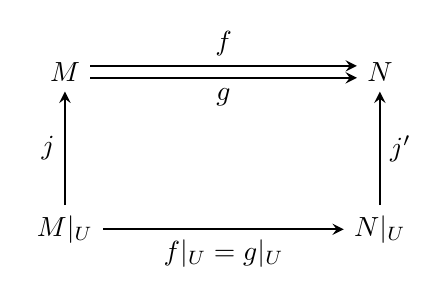
\begin{tikzpicture}[->,>=stealth,thick]  
  \node (A) at (-2,0) {$M|_U$};
  \node (D) at (2,0) {$N|_U$};
  \node (B) at (-2,2) {$M$};
  \node (C) at (2,2) {$N$};

    % Arrows
    \draw[->] (A) -- (B) node[midway, left] {$j$};
    \draw[->] (D) -- (C) node[midway, right] {$j'$};
    \draw[transform canvas={yshift=0.5ex},->] (B) -- (C) node[midway,
    above] {$f$};
    \draw[transform canvas={yshift=-0.5ex},->] (B) -- (C) node[midway,
    below] {$g$};
    \draw[->] (A) -- (D) node[midway, below] {$f|_U=g|_U$};
\end{tikzpicture}
}

\end{frame}


\begin{frame}{Landsman determinism}

\resizebox{0.95\textwidth}{!}{    
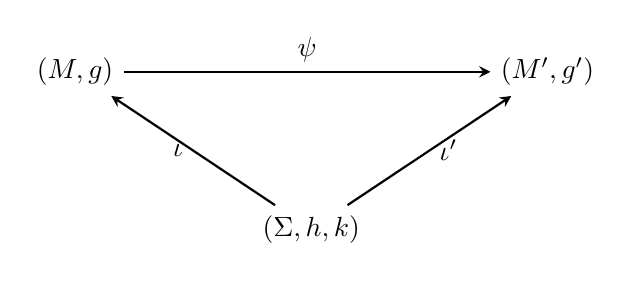
\begin{tikzpicture}[->,>=stealth,thick]
    % Nodes
    \node (A) at (0,0) {$(\Sigma,h,k)$};
    \node (B) at (-3,2) {$(M,g)$};
    \node (C) at (3,2) {$(M',g')$};

    % Arrows
    \draw[->] (A) -- (B) node[midway, left] {$\iota$};
    \draw[->] (A) -- (C) node[midway, right] {$\iota'$};
    \draw[->] (B) -- (C) node[midway, above] {$\psi$};
  \end{tikzpicture}
  }
  
\end{frame}




\begin{frame}{Butterfield-Landsman determinism}

\resizebox{0.7\textwidth}{!}{    
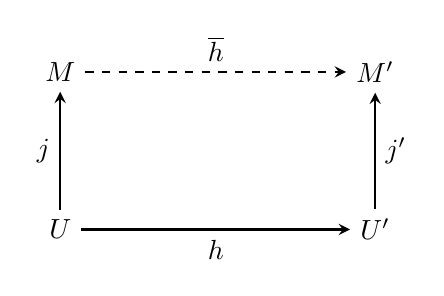
\begin{tikzpicture}[->,>=stealth,thick]
    % Nodes
  \node (A) at (-2,0) {$U$};
  \node (D) at (2,0) {$U'$};
  \node (B) at (-2,2) {$M$};
  \node (C) at (2,2) {$M'$};

    % Arrows
    \draw[->] (A) -- (B) node[midway, left] {$j$};
    \draw[->] (D) -- (C) node[midway, right] {$j'$};
    \draw[dashed, ->] (B) -- (C) node[midway, above] {$\overline{h}$};
    \draw[->] (A) -- (D) node[midway, below] {$h$};
  \end{tikzpicture}
}  

\end{frame}

\begin{frame}{From semantic to syntactic analysis}

  \begin{itemize}
  \item Claim: Let $M,M'$ be models of $T$, and let $h:M\to M'$ be a
    bijection that preserves (i) linking functions, and (ii)
    restricted vocabulary. Then $h$ preserves extensions of full
    vocabulary.
  \item Beth's Theorem: Full vocabulary is definable in terms of
    restricted vocabulary and linking functions.
  \item All facts are \underline{deducible} from facts about an
    initial segment.
  \end{itemize}


\end{frame}

\begin{frame}{How determinism can fail}

  \begin{enumerate}
  \item An isomorphism of initial data does not extend to an
    isomorphism of models.
    \begin{itemize}
      \item Models have more structure than the initial data.
      \item Spontaneous symmetry breaking.
    \end{itemize}
  \item An isomorphism of initial data has more than one distinct
    extension an isomorphism of models.
  \end{enumerate}


\end{frame}

\begin{frame}{MiniMach spacetime}

  Assumptions:
  \begin{itemize}
  \item Two times, two identical spatial points at each time
  \item No relations between points at different times
  \end{itemize}

  \hrulefill

  $T$ is categorical (one model up to isomorphism)

  Initial conditions have a unique extension to a spacetime model.

  But an isomorphism of initial conditions does not uniquely determine
  an isomorphism of models.

  Therefore, $T$ is indeterministic.


\end{frame}

\begin{frame}{Bald philosophers}

  Assumptions:
  \begin{itemize}
  \item There are seven identical, bald philosophers.
  \item At a subsequent time, one of these philosophers grows a hair.
  \end{itemize}

  \hrulefill

  Let $h$ be a permutation of the initial data that exchanges the
  philosopher who will grow a hair with another philosopher.

  There is no isomorphism $\overline{h}$ that extends $h$ to the
  entire model.

  Therefore, $T$ is indeterministic.


\end{frame}

\begin{frame}{White and black spheres}

  Assumptions:
  \begin{itemize}
  \item There are two identical white spheres and two identical black
    spheres
  \item Each white sphere pairs up with a black sphere.
  \item Hence there is a bijection $f$ from white spheres to black
    spheres.
  \end{itemize}

  \hrulefill

  Let $h$ be the automorphism of the domain that fixes the white
  spheres, but flips the black spheres.

  There is no isomorphism $\overline{h}$ that extends $h$ to the
  entire model.

  Therefore, $T$ is indeterministic.

\end{frame}

\begin{frame}{First Order Lessons}

  \begin{itemize}
  \item We appear to have a good definition. It explains the
    difference between GTR (deterministic) and the examples by Belot
    and Melia (indeterministic).
  \item We don't need haecceitism to judge that Belot and Melia's
    examples are indeterministic.
  \item Theories with one model (up to isomorphism) might be
    indeterministic.
  \end{itemize}
\end{frame}

\begin{frame}{First Order Lessons}

  \begin{itemize}  

  \item Theories with unique final conditions (up to isomorphism)
    might be indeterministic. \newline {\small ``Let us say that
      \emph{D-haecceitism} is the view that a theory may be
      indeterministic, even if all the different possible futures open
      to any world which makes the theory true are qualitatively
      identical.'' (Melia 1999, p 640)}
  \item Determinism isn't a matter of identity between worlds or world
    segments.
  \item A theory is deterministic if change of representation of
    initial segments determines a change of representation of entire
    histories.
  \end{itemize}

\end{frame}



\end{document}



\begin{frame}{An indeterministic theory of heat transfer}

  Assumptions:
  \begin{itemize}
  \item Two times, two objects at each time.
  \item At each time, exactly one object is hot.
  \item Objects persist through time.
  \end{itemize}

  \hrulefill

  $T$ has two models up to isomorphism.

  Since each model is rigid, Property R holds.

  An isomorphism between initial conditions cannot necessarily be
  lifted to an isomorphism between models.

  Therefore, $T$ is not Landsman deterministic.



\end{frame}






\begin{frame}

  Perhaps the previous example doesn't seem indeterministic.

  There is only one way things can be at the latter time.


\end{frame}

\begin{frame}{Theory: There can only be one}

  Assumptions
  \begin{itemize}
  \item At $t=0$ two particles exist. 
  \item At $t=1$ exactly one of those two particles still exists.
  \end{itemize}

  Formalized via a relation $\delta$ that holds between the particles
  at $t=0$ and the particle at $t=1$

  

\end{frame}

\begin{frame}{Version 1}

  $T_1$ has no non-trivial predicates that apply to the domain at
  $t=0$.

  \hrulefill

  $T_1$ is categorical, and its unique model is rigid. (The function
  $\delta$ selects one of the particles.)

  Therefore, $T_1$ is Landsman deterministic.


\end{frame}

\begin{frame}{Version 2}

  $T_2$ has predicates $L$ and $R$ that apply to the domain at $t=0$.

  \hrulefill

  There is a unique initial condition, up to isomorphism.

  There is a unique final condition, up to isomorphism. 

  $T_2$ has two non-isomorphic models: one in which $L$ survives, and
  one in which $R$ survives.

  Therefore, $T_2$ is Landsman indeterministic.

\end{frame}




\end{document} 
%%% Local Variables:
%%% mode: latex
%%% TeX-master: t
%%% End:
